\section{Experiments}
\label{task:evaluation}

To gauge the impact of our changes, we tested our functional conversion (New) against the untyped one (Old) on several relations. 
The new pipeline matches the old in every case and improves upon it in presence of semi-deterministic relations. 
We consider three relations: addition, generating permutations as a reverse of sorting, and typechecking used to enumerate terms of a given type. 
These relations showcase different aspects of performance gains.

\begin{figure}[ht]
\makebox[\textwidth][c]{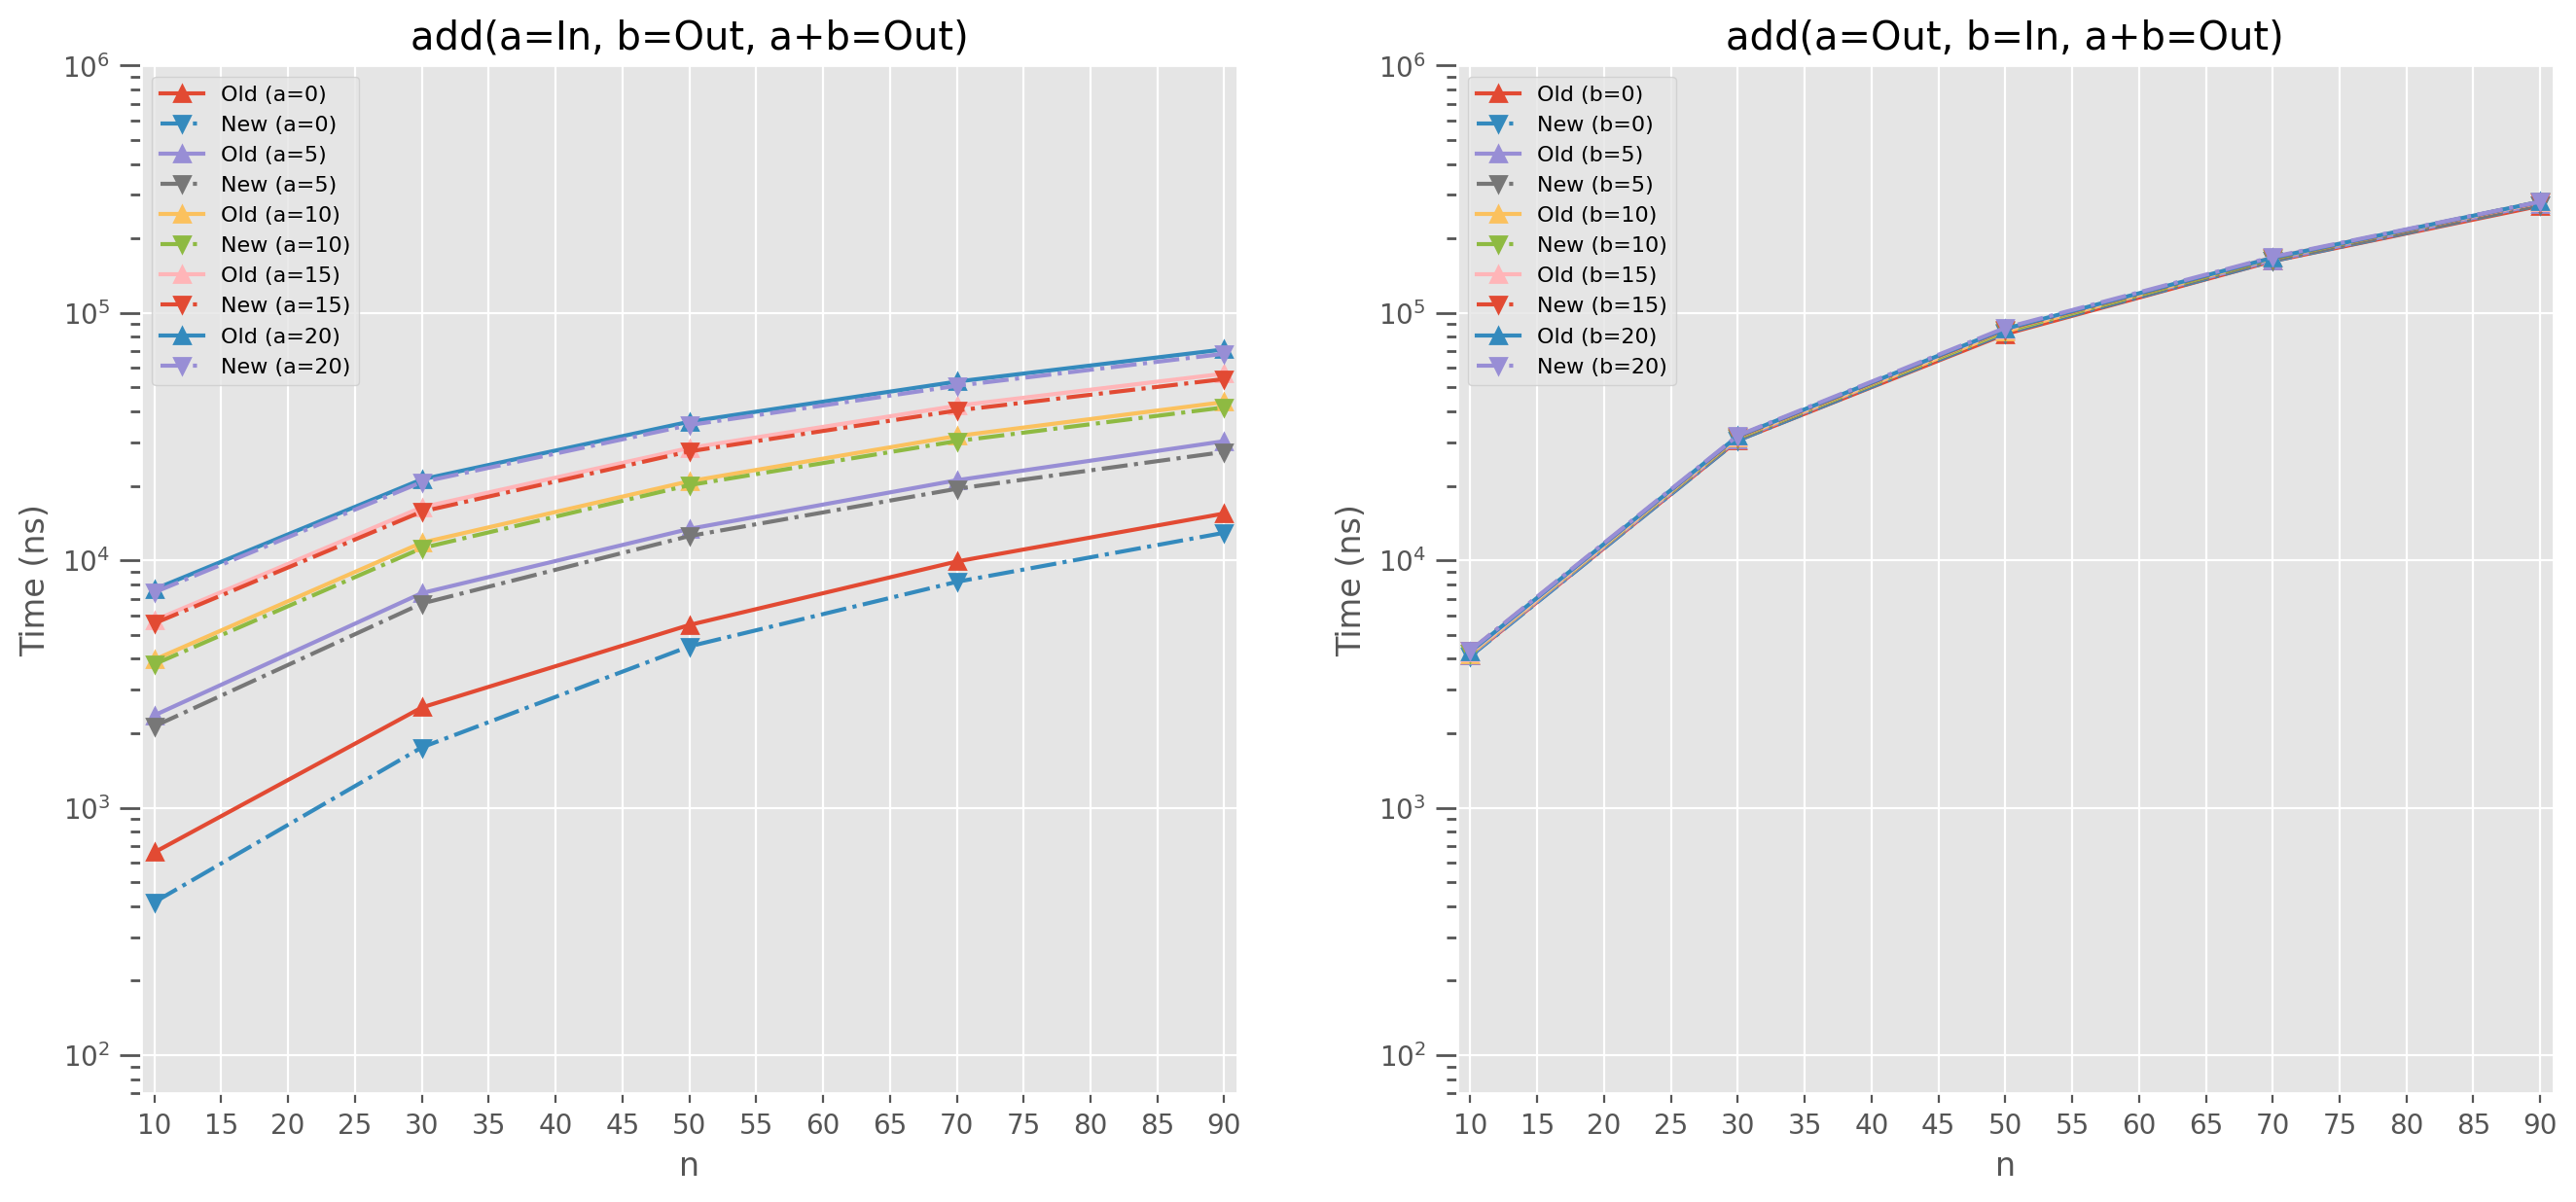
\includegraphics[width=0.9\textwidth]{./img/addNondet.png}}
\caption{Execution time (in nanoseconds) of $add$ relation in two nondeterministic directions, requesting first $n$ (x-axis) results. Log plot.}
\label{fig:addNondet}
\end{figure}


\begin{figure}[h!]
\makebox[\textwidth][c]{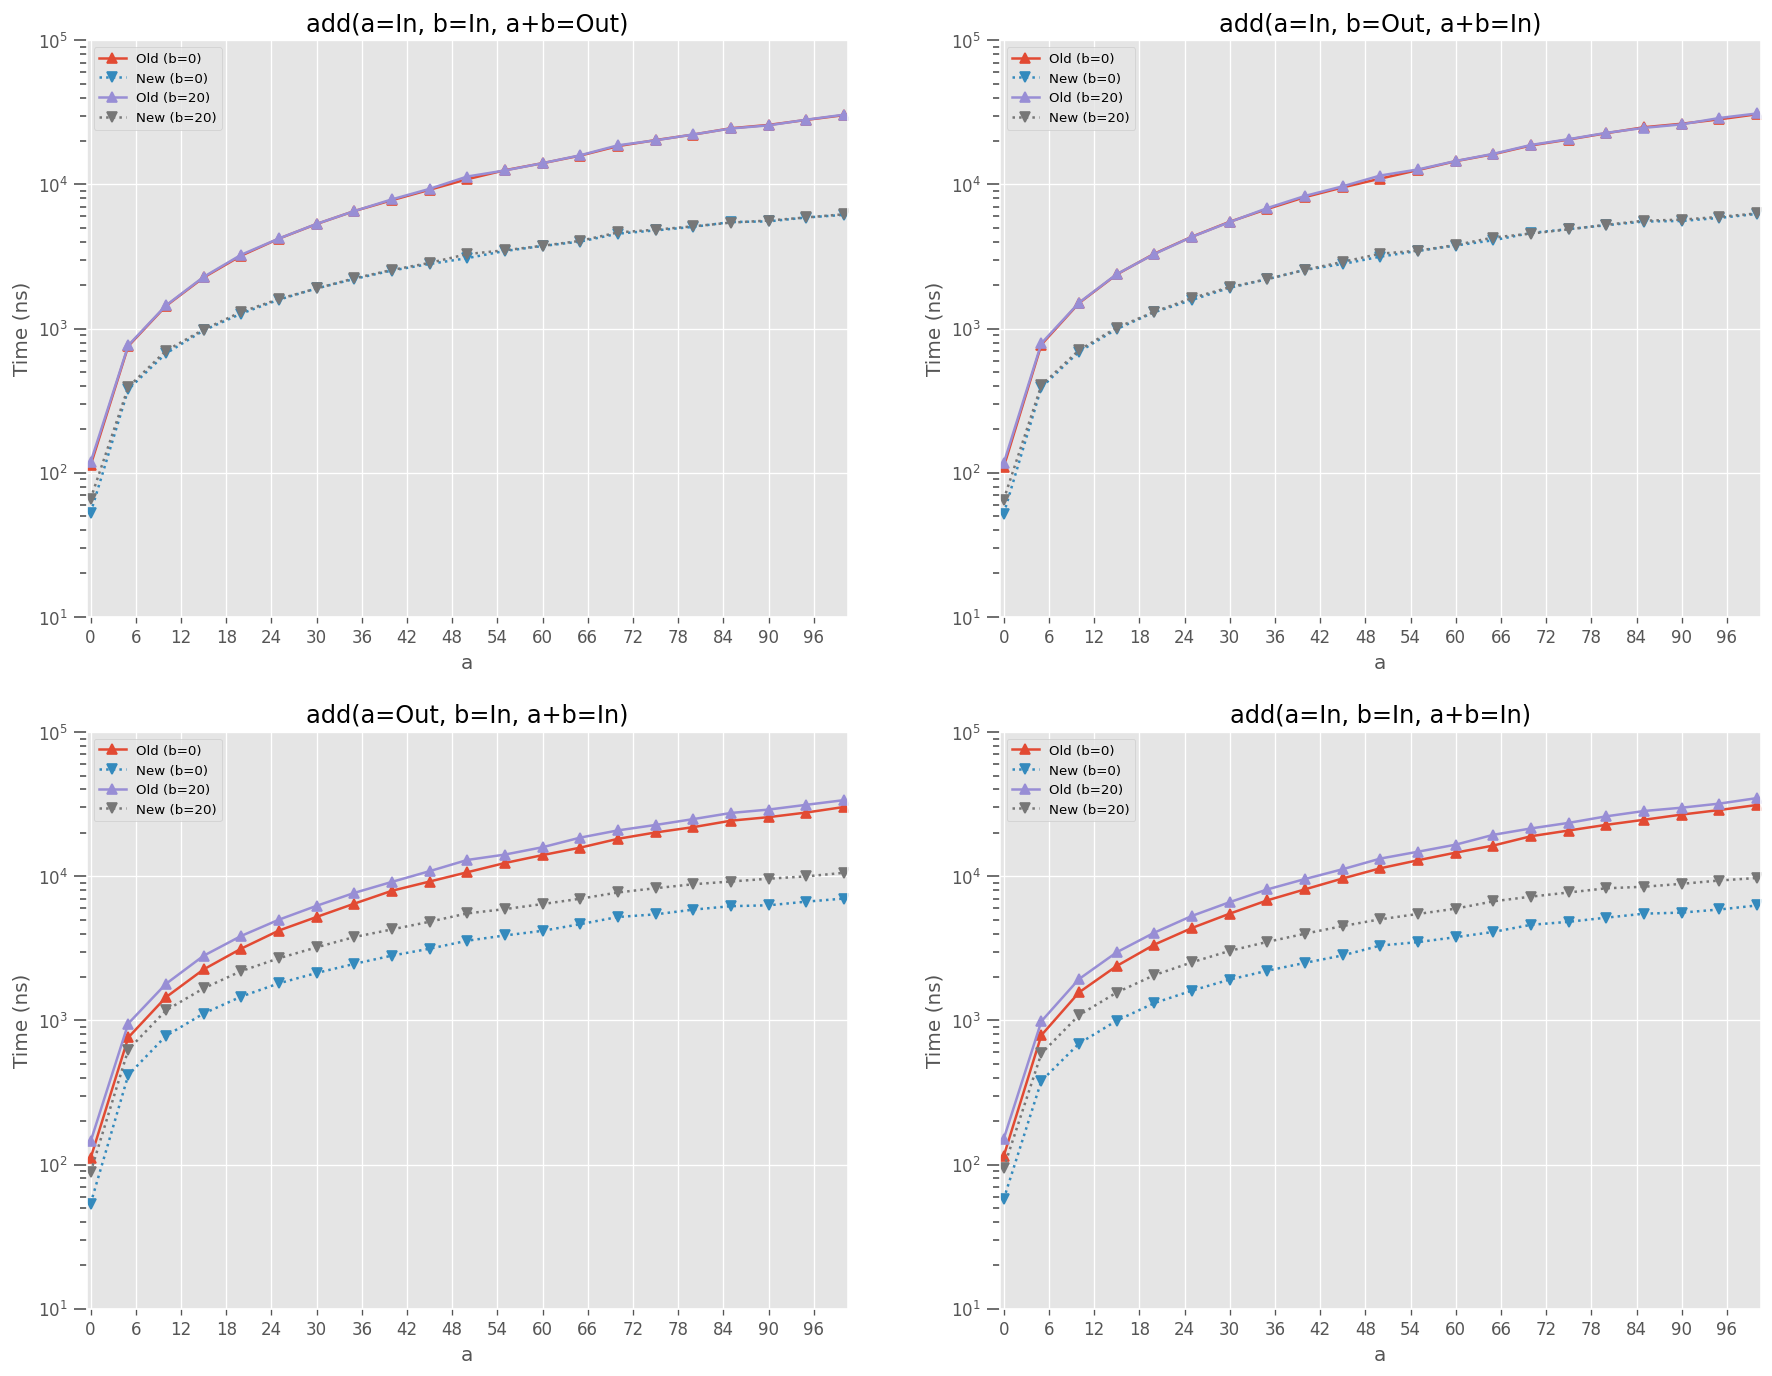
\includegraphics[width=0.9\textwidth]{./img/addDet.png}}
\caption{Execution time (in nanoseconds) of $add$ relation in four deterministic directions, with parameter $a$ on x-axis. Log plot.}
\label{fig:addDet}
\end{figure}

Figure \ref{fig:addNondet} presents nondeterministic directions of addition, when exactly one variable is known. 
In the direction $R_{\text{add}}\left( \In, \Out, \Out \right)$ the relation uses one generator, and shows slight speed-up. 
The $R_{\text{add}}\left( \Out, \In, \Out \right)$ direction does not feature any optimization opportunities for our improved converter since it is nondeterministic, uses a single type, and avoids using generators. 
As a result, its performance matches the old implementation exactly.


Figure \ref{fig:addDet} covers semi-deterministic directions of addition.
A clear performance improvement can be observed across all functions,
reaffirming the importance of tracking determinism.

\begin{figure}[ht]
\makebox[\textwidth][c]{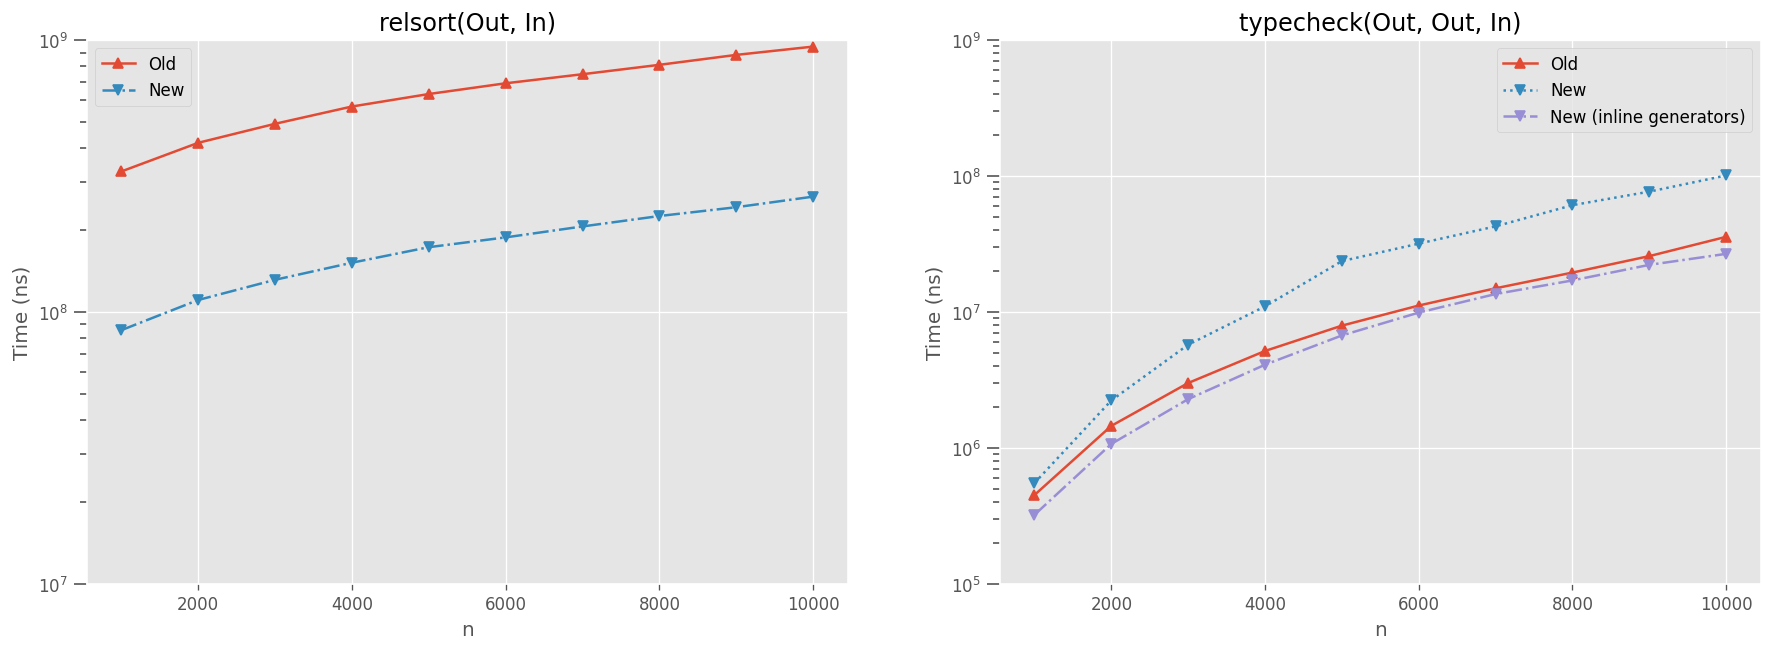
\includegraphics[width=0.9\textwidth]{./img/sorttypecheck.png}}
\caption{Execution time (in nanoseconds) of generating permutations from $12$-element list with the $sort$ relation and enumerating terms and contexts that infer to a given type by the $typecheck$ relation, requesting first $n$ (x-axis) results. Log plot.}
\label{fig:sorttypecheck}
\end{figure}

The left panel of Figure \ref{fig:sorttypecheck} showcases generating permutations of a sorted $12$-element list by the \emph{sort} relation. 
We observe performance improvement which arises entirely from semi-determinism of comparison relations.

The right panel of Figure \ref{fig:sorttypecheck} utilizes the $typecheck$ relation to enumerate terms of a simple expression language that type check to the \emph{Integer} type. 
This example demonstrates the importance of using \lstinline{INLINEABLE} annotation for generators. 
When they are correctly inlined, we observe a reduced execution time, while naive implementation only worsens performance. 

Overall, the new converter never slows down the relations. 
Moreover, in some cases, determinism analysis yields qualitative improvements by identifying computations which can safely be pruned once a single answer has been produced. 